\documentclass[tikz]{standalone}
% Where edge labels sit (M2b follow-up, D57). Each label is a named node, so
% the interpreter can be checked against pdfTeX: `auto` and `auto, swap` on
% level, upright, diagonal and curved segments, on both pieces of `|-` and
% `-|` and at several `pos` values, against the plain `above`/`left` keys
% that only suit one orientation.
\tikzset{every node/.style={draw, minimum width=1cm, minimum height=6mm}}
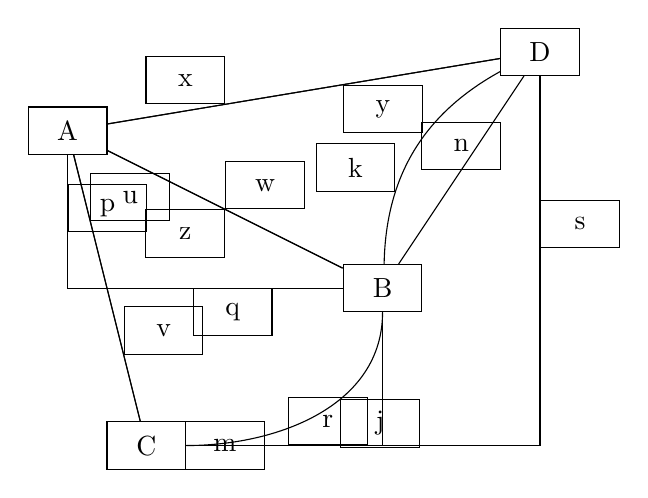
\begin{tikzpicture}
  \node (a) at (0,0) {A};
  \node (b) at (4,-2) {B};
  \node (c) at (1,-4) {C};
  \node (d) at (6,1) {D};
  % level, upright and diagonal lines, both directions
  \draw (a) -- node[auto, name=l1, pos=0.3] {x} (d);
  \draw (a) -- node[auto, swap, name=l2, pos=0.6] {y} (d);
  \draw (a) -- node[auto, name=l3, near start] {u} (c);
  \draw (c) -- node[auto, swap, name=l4, near start] {v} (a);
  \draw (a) -- node[auto, name=l5] {w} (b);
  \draw (b) -- node[auto, name=l6] {z} (a);
  % both pieces of orthogonal paths, left and right
  \draw (a) |- node[auto, name=l7, pos=0.2] {p} (b);
  \draw (a) |- node[auto, swap, name=l8, pos=0.8] {q} (b);
  \draw (c) -| node[auto, name=l9, pos=0.2] {r} (d);
  \draw (c) -| node[auto, swap, name=l10, pos=0.8] {s} (d);
  % the keys that only suit one orientation
  \draw (b) |- node[left, name=l11, pos=0.8] {m} (c);
  \draw (b) -- node[above, name=l12, pos=0.5] {n} (d);
  % curves
  \draw (b) to[bend left] node[auto, name=l13, pos=0.3] {k} (d);
  \draw (c) to[out=0, in=270] node[auto, swap, name=l14, pos=0.6] {j} (b);
\end{tikzpicture}
